

\begin{figure}
	\centering
	\begin{minipage}{.5\textwidth}
	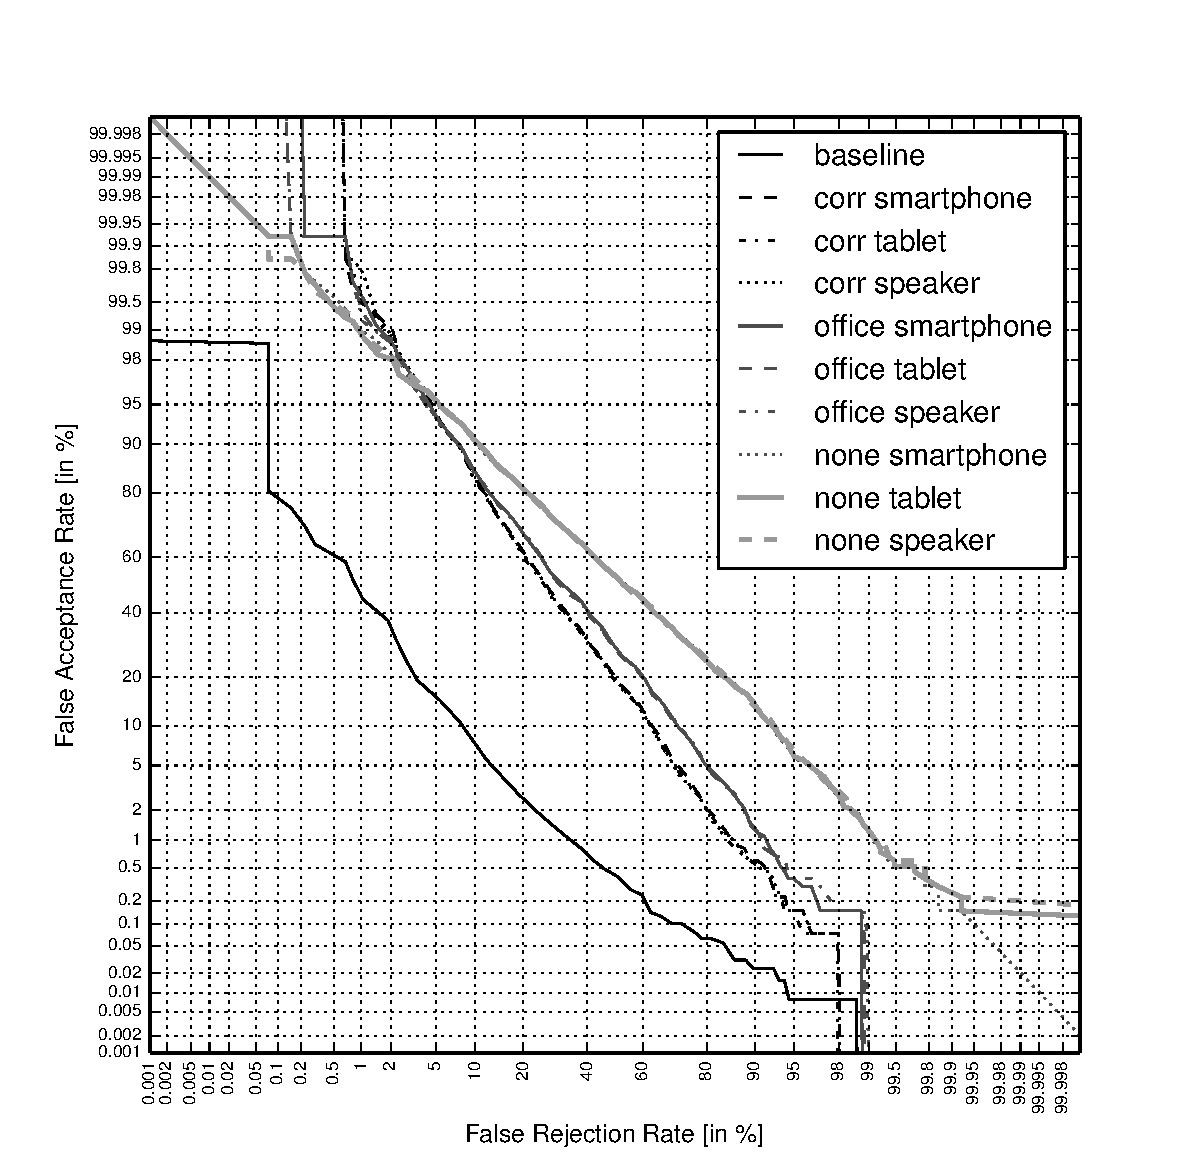
\includegraphics[width=1\linewidth]{Figs/DETs_GMM.pdf}
	\caption{DET plots for the GMM-UBM system for various replay configurations, compared to the baseline performance.}
	\label{fig::DETs_replay_GMM}
	\end{minipage}
	\begin{minipage}{.5\textwidth}
	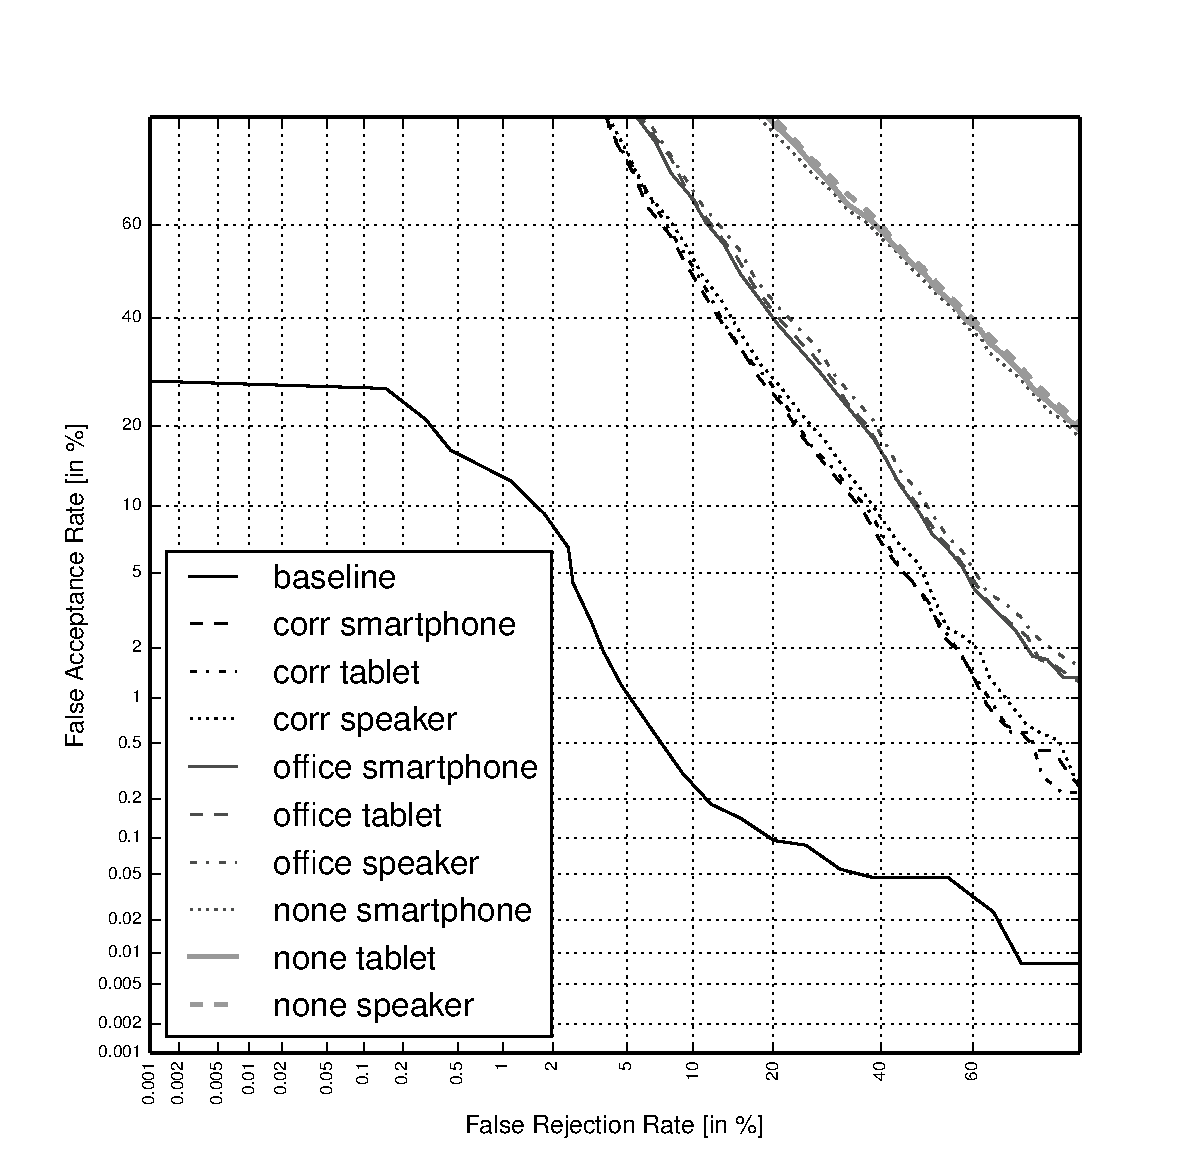
\includegraphics[width=1\linewidth]{Figs/DETs_IV.pdf}
	\caption{DET plots for the IV-PLDA system for various replay configurations, compared to the baseline performance.}
	\label{fig::DETs_replay_IV}
	\end{minipage}


\end{figure}



\begin{figure}
	\centering
	\begin{minipage}{.5\textwidth}
	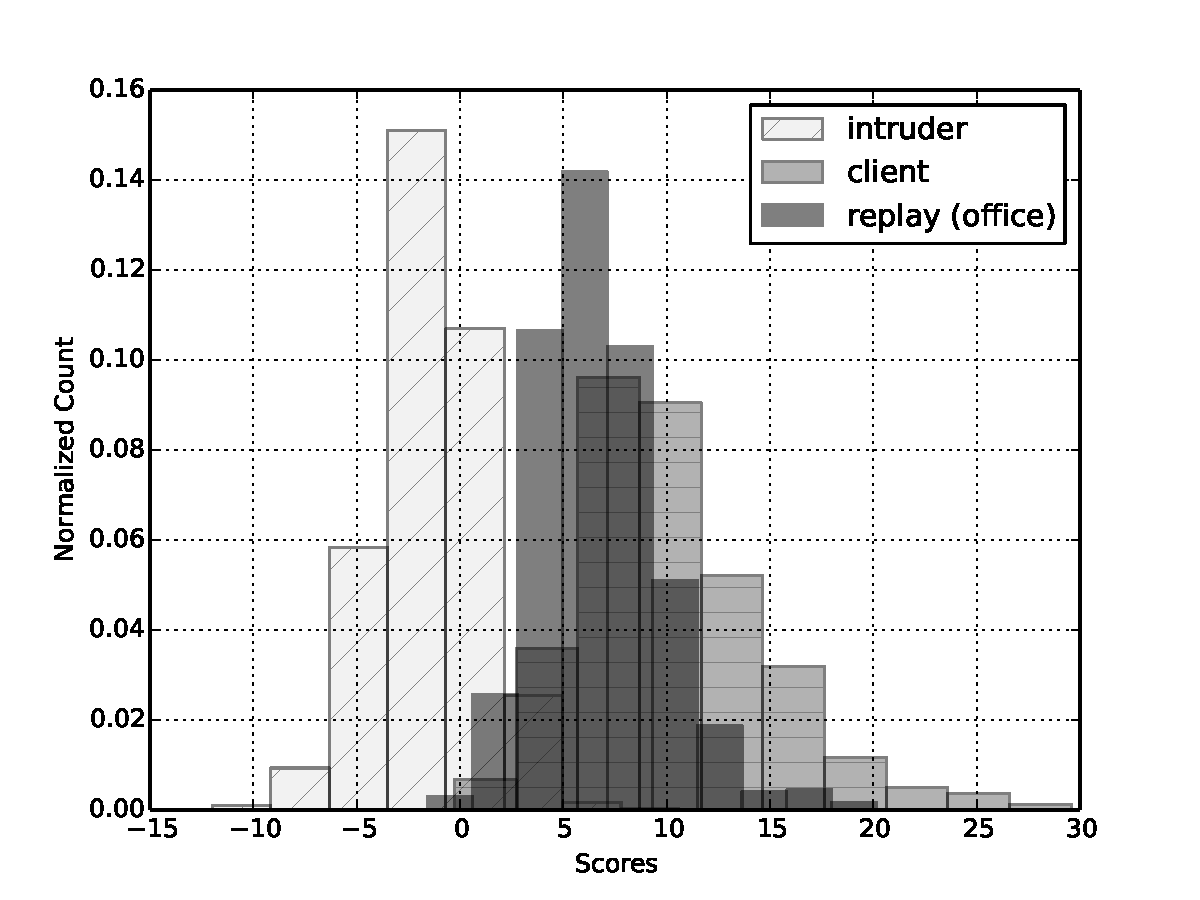
\includegraphics[width=1\linewidth]{Figs/dist_IV_off.pdf}
	\end{minipage}

%	\begin{minipage}{0.5\textwidth}
%	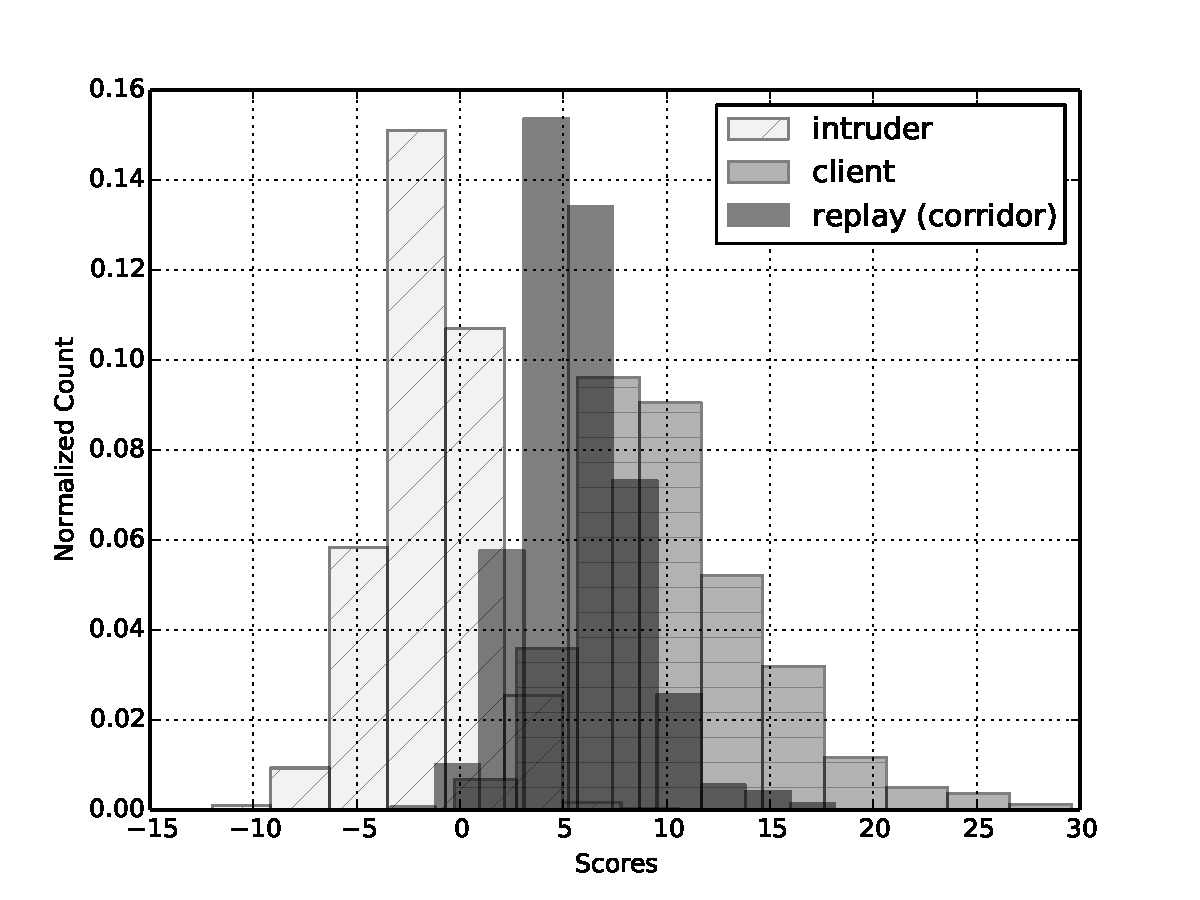
\includegraphics[width=1\linewidth]{Figs/dist_IV_corr.pdf}
%	\end{minipage}
%
%	\begin{minipage}{0.5\textwidth}
%	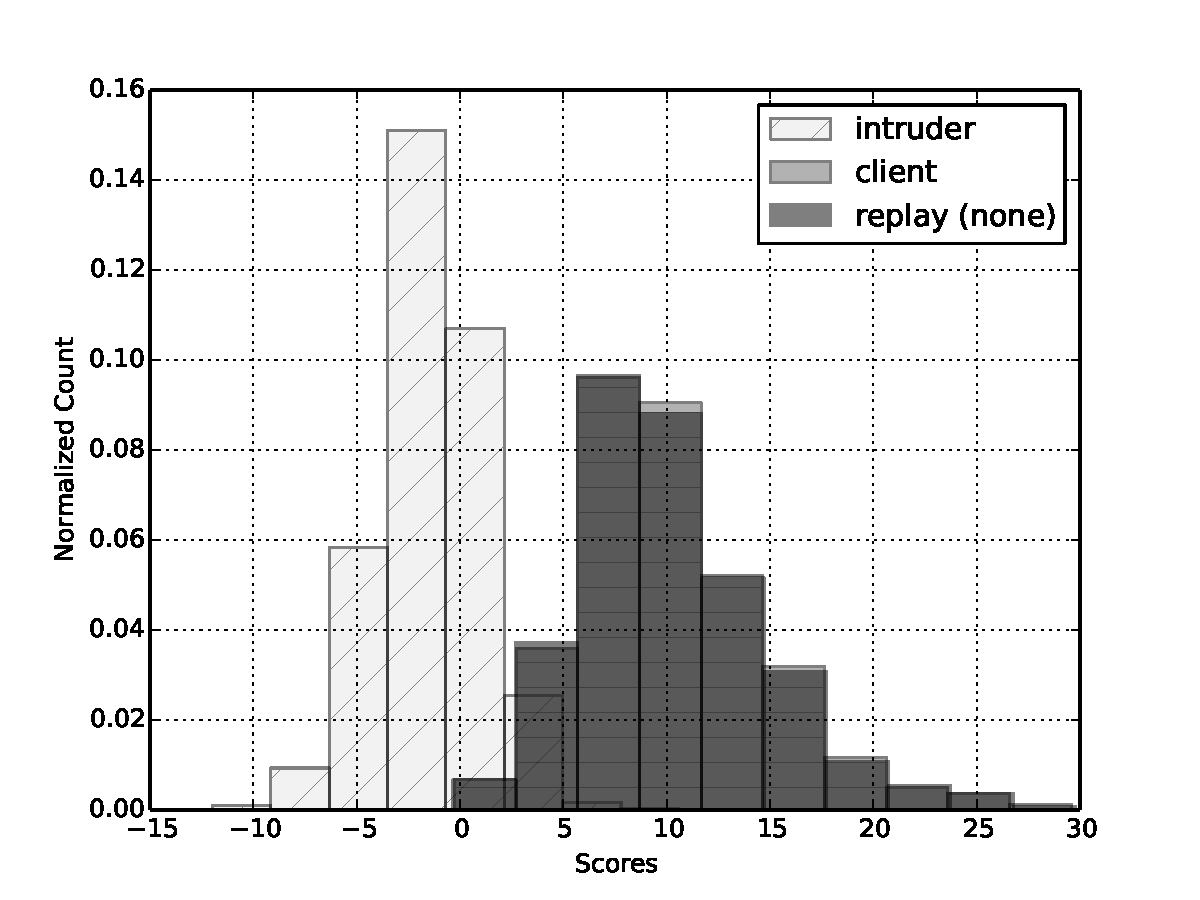
\includegraphics[width=1\linewidth]{Figs/dist_IV_none.pdf}
%	\end{minipage}

	\caption{Score distribution for the IV-PLDA system for replay attacks using a stand-alone speaker and with simulation of an office.}
	\label{fig::Dist_IV}
\end{figure}

%DETs described
Fig.~\ref{fig::DETs_replay_GMM} and Fig.~\ref{fig::DETs_replay_IV} present the detection error trade-off (DET) plots\footnote{Produced with the TABULA RASA Scoretoolkit (http://publications.idiap.ch/downolads/reports/2012/Anjos\_Idiap-Com-02-2012.pdf)}  for the basic GMM-UBM and the state-of-the-art IV-PLDA systems, exposed to various replay attacks. They show that all replay attacks caused a significant degradation of the ASV performance. However, there are major differences in ASV performance depending on acoustic environment. If the acoustic environment is omitted, the ASV system is almost ideally spoofed -- the DET lines are close to straight, with the EER values close to 50\%. In realistic cases, when the room acoustics is taken into account, the spoofing is slightly less severe. It can be easily observed that the ASV performance under replay attack in a corridor is better than in an office, probably due to higher level of reverberation for the corridor. 

These results are confirmed by score distribution presented in Fig.~\ref{fig::Dist_IV} -- they show that without considering the acoustic environment (the bottom plot) the scores for replay attacks overlap the scores of genuine client accesses, whilst the scores returned by the IV-PLDA system with a replay attack realised in a corridor (or with speech acquired in a corridor) are shifted towards impostor trials, however still with a significant overlap with true client accesses (see the middle plot of Fig.~\ref{fig::Dist_IV}).

In contrast, despite major differences in speakers' impulse responses (see Fig.~\ref{fig::IRs}), the differences between the DET plots corresponding to different speakers are only minor. It suggests a relatively low impact of a replay device on the effectiveness of replay attack. Since all seven ASV systems tested showed similar behaviour, therefore, for the sake of clearness, the next results will present the average of the three speakers used in experiments.




%EER table described
Table~\ref{tab::results_EER} shows the detailed EER results for replay attacks in various acoustic conditions against the seven various ASV systems, with and without score normalisation. All systems are shown to be severely sensitive to replay attacks. Even for the highly-reverberant corridor and the most resistant (in terms of EER) GSL kernel system with factor analysis and with T-norm, the EER rose to more than 22\% compared to the baseline 5.7\%. What was already visible in the DET plots (see Fig.~\ref{fig::DETs_replay_IV}), the results for the office are much worse -- the most resistant IV system (without PLDA and without score normalisation) and GSL-FA systems yielded the EER of ca. 28\%, whilst the other systems returned EERs of 30\% and more. If acoustic conditions are not emulated, the spoofing is almost perfect and the ASV systems yield EER values of 50\% or even more. 


\begin{figure}
	\centering
	\begin{minipage}{.5\textwidth}
	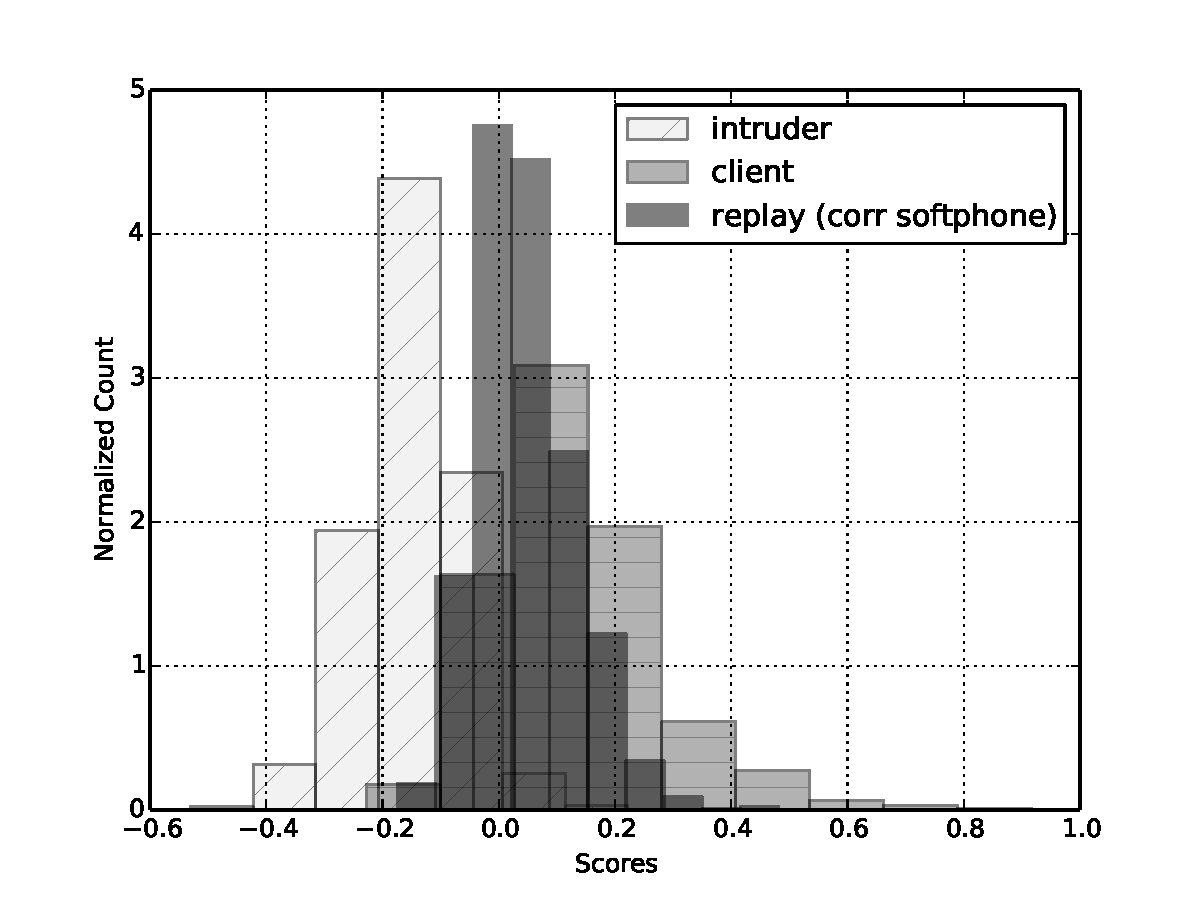
\includegraphics[width=1\linewidth]{Figs/dist_GMM_corr_iPhone.pdf}
%	\caption{DET plots for GMM-UBM (left) and i-Vectors-PLDA (right) systems.}
%	\label{fig::Dist_GMM_corr}
	\end{minipage}


	\begin{minipage}{0.5\textwidth}
	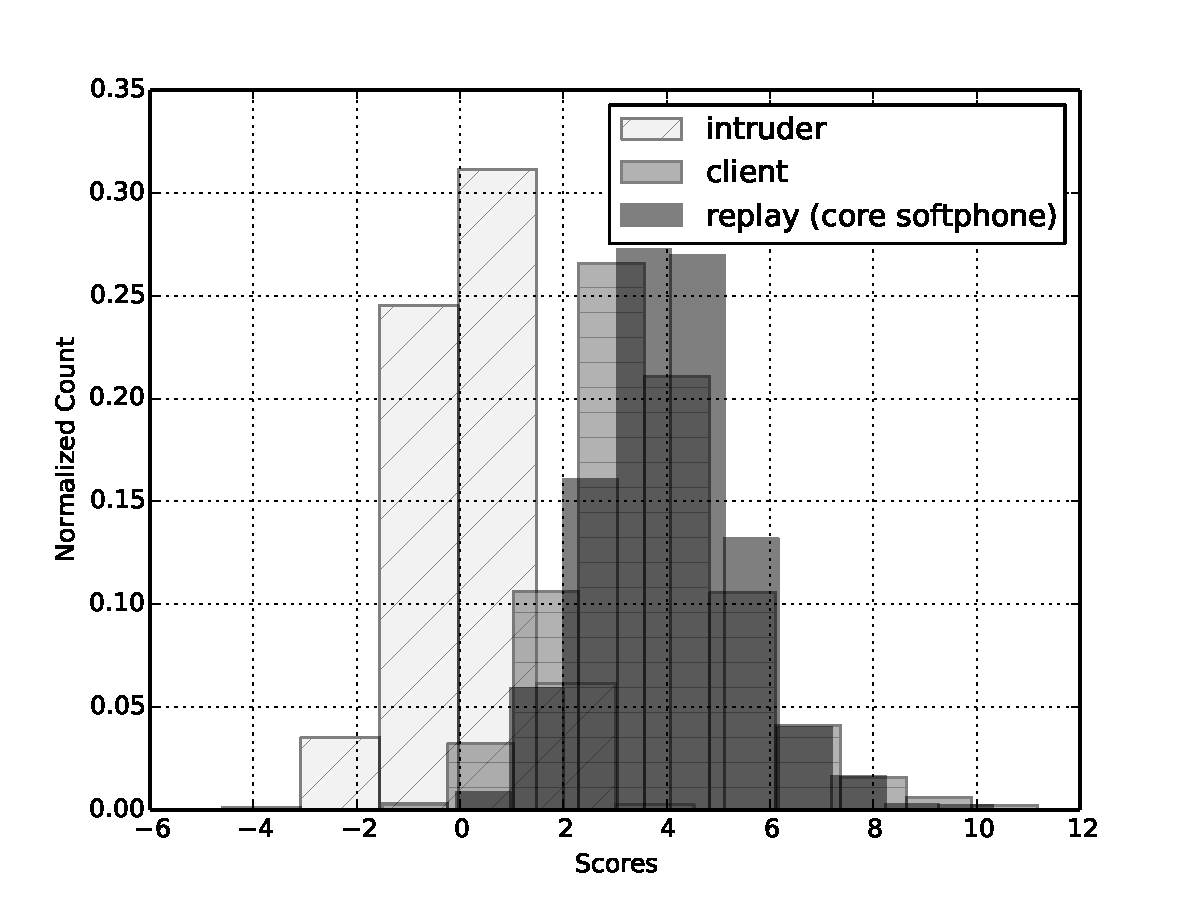
\includegraphics[width=1\linewidth]{Figs/dist_GMM_T_corr_iPhone.pdf}
%	\caption{DET plots for iVectors-PLDA xxxxxxxxxxxxxxxxxxx}
	\end{minipage}

	\caption{Score distribution for the GMM-UBM system without (top) and with (bottom) score normalisation.}
	\label{fig::Dist_GMM.T_corr}

\end{figure}



%% comparison with other attacks
\subsection{Comparison of replay threat vs. other spoofing methods}

\begin{table*}
%\ninept
\begin{center}
    \begin{tabular}{ l || c c c c c c}
    \hline
     	 Attack & GMM & SGL & SGL-NAP & SGL-FA & FA & IV-PLDA \\ 

 \hline \hline
Na\"{i}ve impostor & 9.08 & 7.89 & 6.35 & 6.08 & 5.60 & 3.20\\ 
Replay & 37.99	& 31.33 & 31.03 & 28.24 & 31.89 & 25.95\\
Voice conversion & 31.48 & 36.94 & 30.44 & 30.23 & 23.16 & 20.45\\ 
Speech synthesis & 39.90 & 14.66 & 13.83 & 11.98 & 30.81 & 10.92\\ 
\hline
    \end{tabular}
    \caption{EER values for different ASV systems for various spoofing attacks, without score normalisation.}
		\label{tab::results_EER_4attacks}
   \end{center}
\end{table*}


\begin{figure}
	\centering
	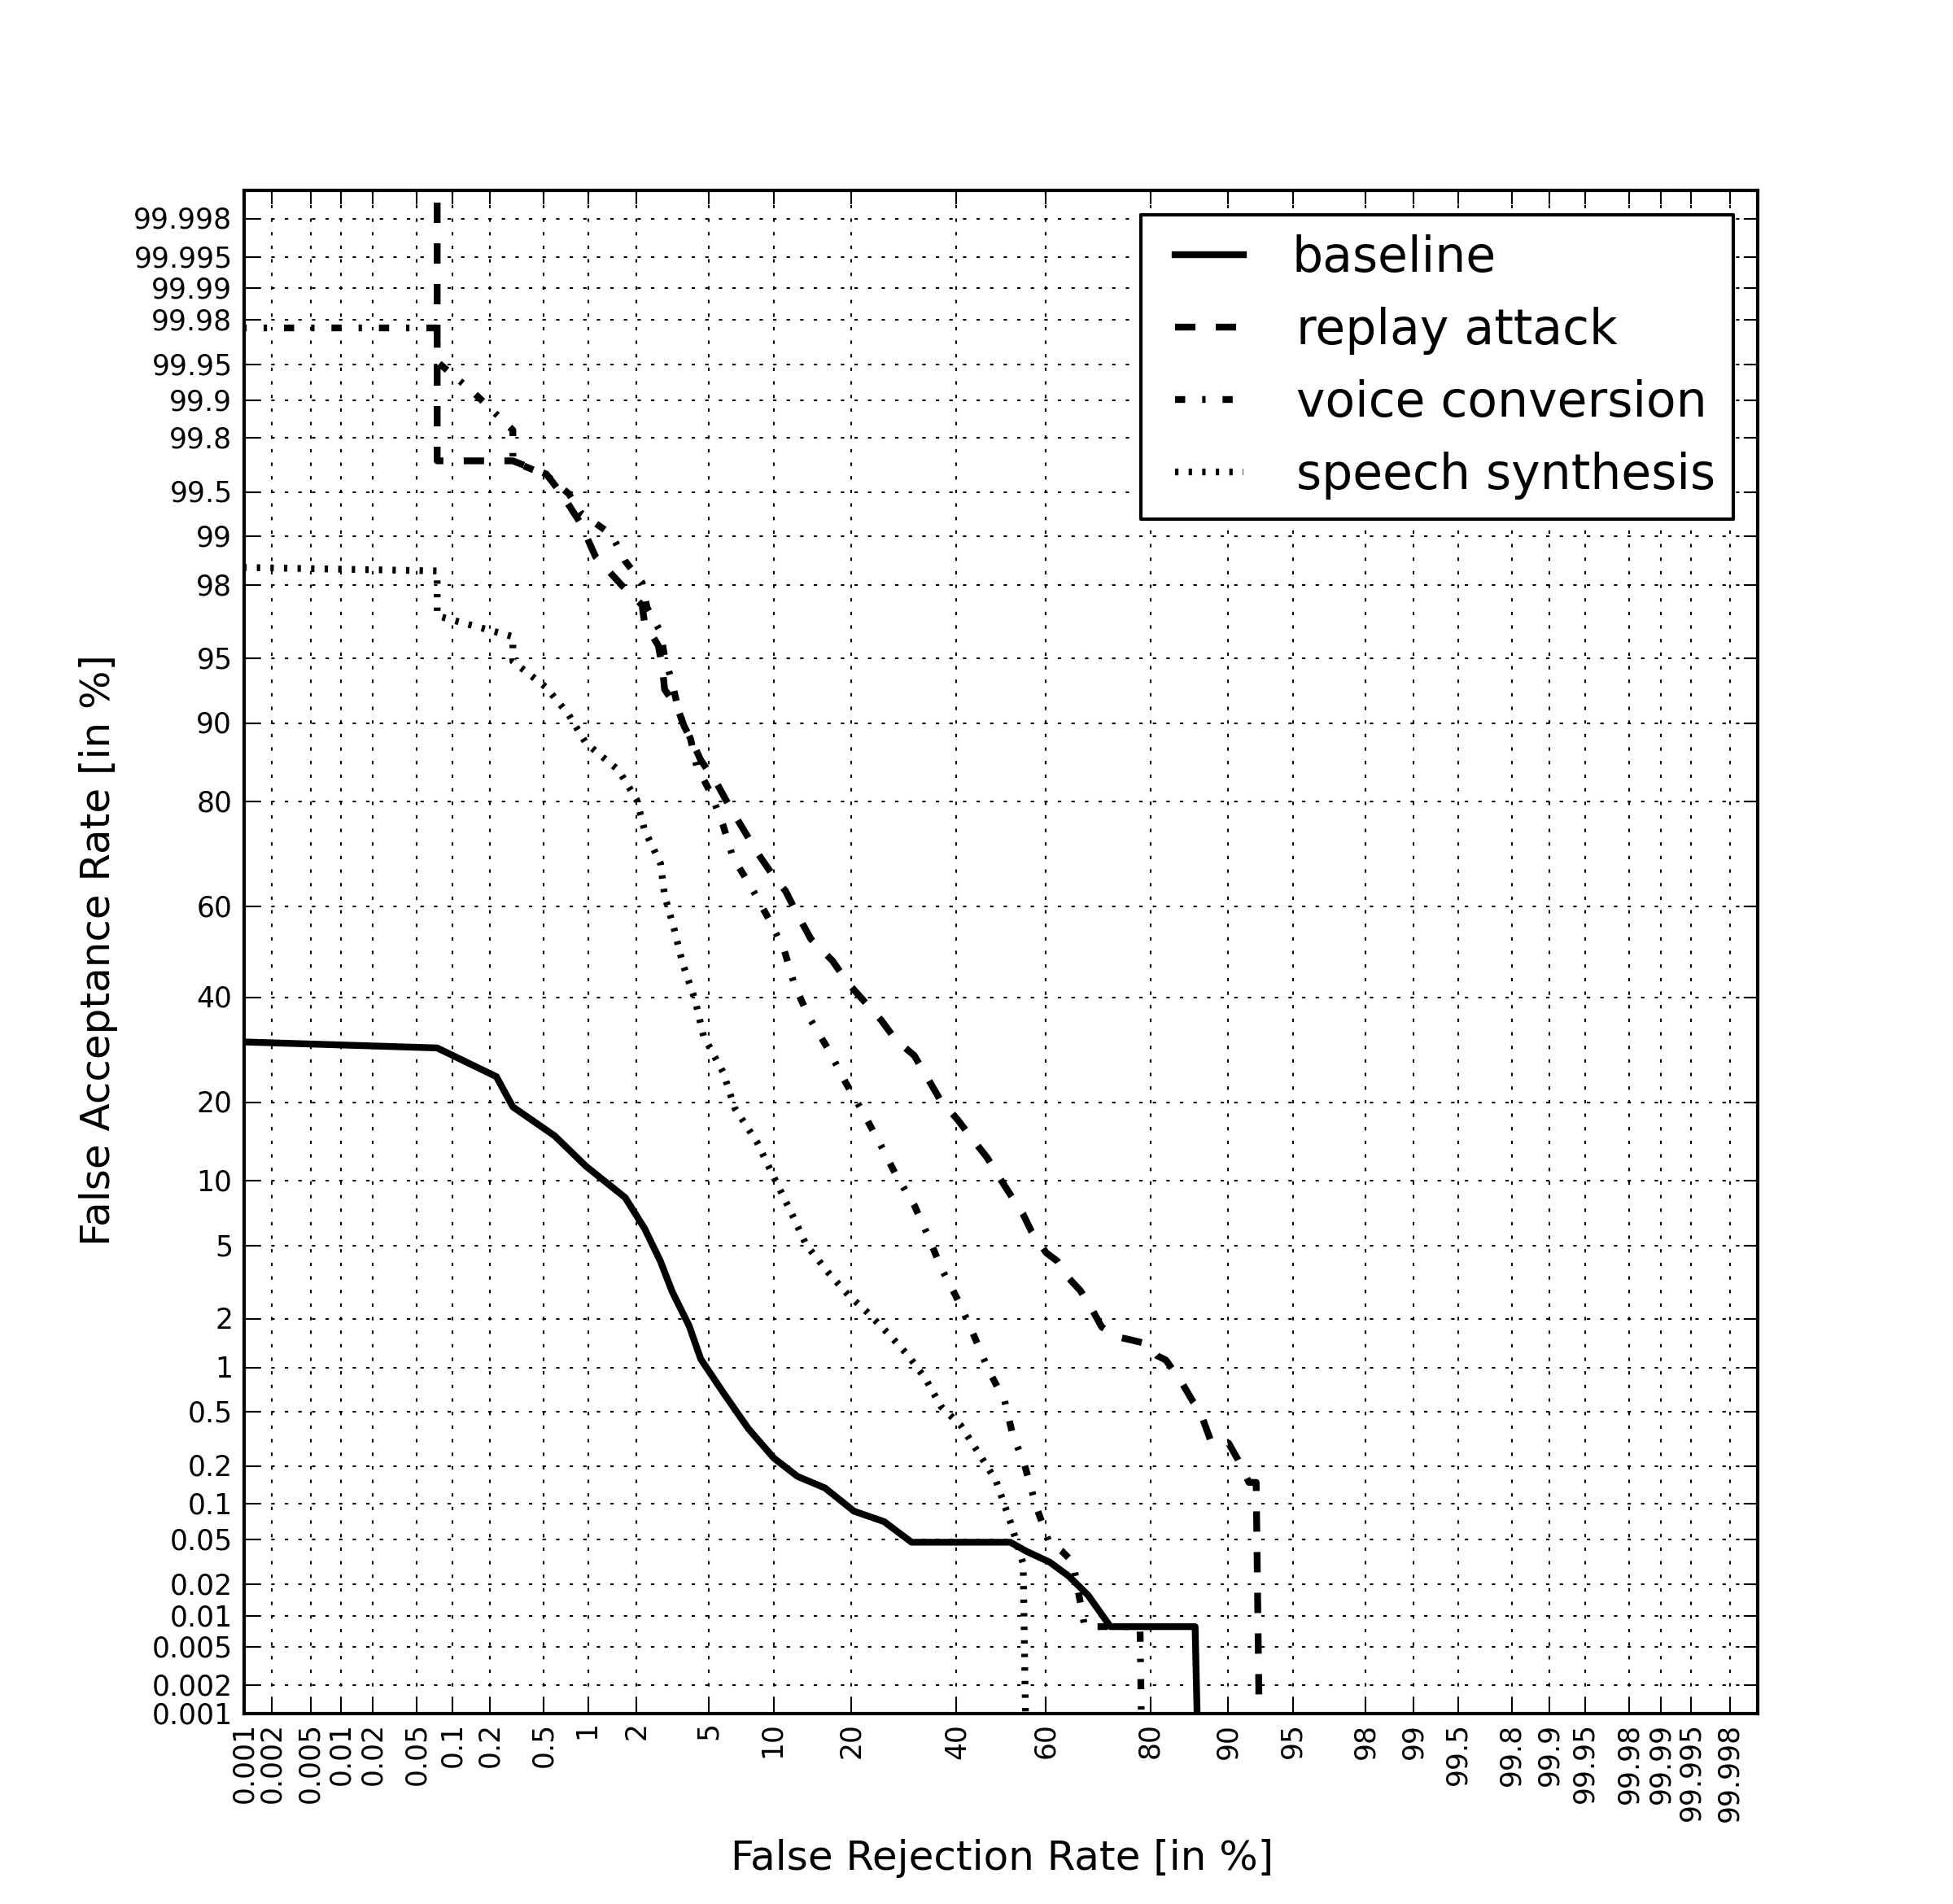
\includegraphics[width=1\linewidth]{Figs/DET_IV_ss_vc_rp.png}
	\caption{DET plots for iVector-PLDA system and various attacks.}
	\label{fig::DETs_4attacks}
\end{figure}

To compare the reply threat with the threat of voice conversion and speech synthesis, we took the average results for all replay devices, as well as the average for office and corridor as the replay environment.
The impact of voice conversion, despite demanding considerably more effort to implement, causes a similar degradation in performance to that of replay attacks. E.g., the SGL system yielded the EER of 37\% for voice conversion and on average 31\% for replay; in contrast, the IV-PLDA system showed to be more resistant to voice conversion than replay (20.5\% EER vs. 26\%, respectively). 

High-effort speech synthesis attacks proved much less effective -- the EER for the best IV-PLDA system reached less than 11\%, whilst replay attack caused an increase of the EER to 20.5\%. These observations are also illustrated through the DET plot in Fig.~\ref{fig::DETs_4attacks} for the IV-PLDA system.

%IN CONTRAST, it turns out that..... (REFERENCE TO BIOSIG PAPER ~\cite{Alegre2014}, SUMMARY OF THE RESULTS from THERE)
% displays... TBC.



\subsection{Impact of score normalisation}

The impact of score normalisation in the case of replay attack is ambiguous.  For some of the systems, such as factor analysis, GMM supervector linear kernel with factor analysis and with nuisance attribute projection the score normalisation helped to decrease EER values in the face of spoofing, e.g., for the factor analysis system and the corridor the EER decreased from almost 30\% to around 25\%. 

\begin{figure}
	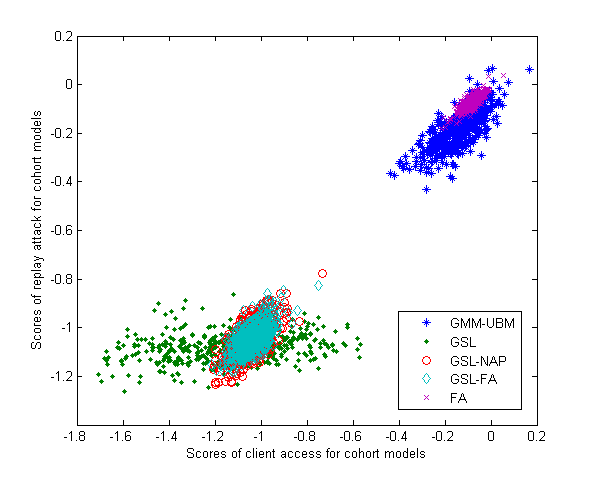
\includegraphics[width=1\linewidth]{Figs/Scores_cohort.png}

	\caption{Score distribution for replay attacks vs. client accesses calculated against cohort speaker models, for various ASVs.}
	\label{fig::Scores_cohort}
\end{figure}

In contrast, for four other ASV systems (GMM-UBM, GMM supervector linear kernel alone and both iVector systems), the score normalisation in fact helped the spoofer. The increase of EER after applying score normalisation for the GMM-UBM or SGL system is immense, e.g., for replay in an office and the GSL system, the EER increased from 34\% to 93\%. This effect is also well illustrated by score distributions presented in Fig. \ref{fig::Dist_GMM.T_corr}, using the example of replay played back from a smartphone in a corridor against a GMM-UBM system. It shows that the scores, having been normalised, got shifted even more to the right than original client accesses. 

This phenomenon seems to be a side-effect of T-norm algorithm, which involves dividing the scores by standard deviation of the scores reached for a cohort of reference speaker models. Table~\ref{tab::scores_cohort} displays standard deviation values for the client accesses and replay spoofed accesses. It shows that standard deviation for client accesses is by far the largest for the GMM supervector linear kernel system (0.25) and it is also relatively high for the GMM-UBM system (0.09). We believe that this is caused by lack of any compensation mechanism for channel and intersession variability, both in the GMM-UBM and the GSL systems. Higher standard deviation causes shifting the scores of the licit client accesses to the left on the score axis. Contrary, other ASVs cause much lower score dispersion (0.06 or less), what is also visible in Fig.~\ref{fig::Scores_cohort}. 

In contrast, standard deviation of scores for replay attacks is pretty low (0.07 or less, see Table~\ref{tab::scores_cohort}) -- this makes the normalised scores increase, so this is why they are shifted to the right in Fig.~\ref{fig::Dist_GMM.T_corr}, and this is why such systems are so vulnerable to replay attacks. This may pose a significant risk to those ASV systems facing a replay attack.

\begin{table}
%\ninept
\begin{center}
    \begin{tabular}{ l || c c c c c }
    \hline
     	 Scores/ASVs & GMM & GSL & GSL-NAP & GSL-FA & FA\\ 

 \hline \hline
Client accesses & 0.086 & 0.252 & 0.063 & 0.057 & 0.032\\
Replay attacks & 0.072 & 0.060 & 0.068 & 0.059 & 0.027\\
\hline
    \end{tabular}
    \caption{Standard deviation of client access scores calculated against cohort speaker models during score normalisation.}
		\label{tab::scores_cohort}
   \end{center}
\end{table}


\subsection{Impact of using PLDA with iVector systems}

When analysing operation of various ASV systems, we also compared the performance of both iVector systems used in experiments - with and without probabilistic linear discriminant analysis (PLDA). The results in Table~\ref{tab::results_EER}, confirmed by Fig.~\ref{fig::EER_PLDA}, clearly show that even though the PLDA significantly decreases the EER for the baseline system (from 6.7\% down to less than 3\%, with score normalisation), it mostly increases the EER when under replay attack. E.g., for an office and score normalisation the EER rose from less to 29\% to 30.3\%. 

%Similar tendency can be seen in DET plots shown in Fig.~\ref{fig::DETs_PLDA}. 

This behaviour of PLDA can be explained as follows: in normal conditions the PLDA improves significantly the performance of iVector-based ASV system as it compensates the intersession differences caused by channel or speaker variation. However, in the case of replay attack this can be disadvantageous, because it also seems to compensate the differences caused by replay devices and replay environments.

%% EER w/wo PLDA
\begin{figure}
	\centering
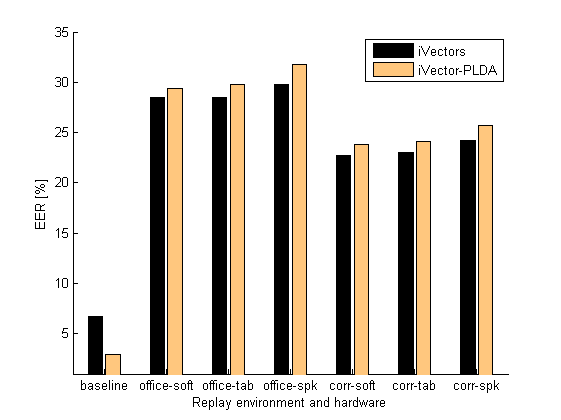
\includegraphics[width=1\linewidth]{Figs/EER_PLDA.png}
	\caption{EER results for iVector-based ASV system with and without PLDA, with score normalisation used.}
	\label{fig::EER_PLDA}
\end{figure}


%\begin{figure}
%	\centering
%	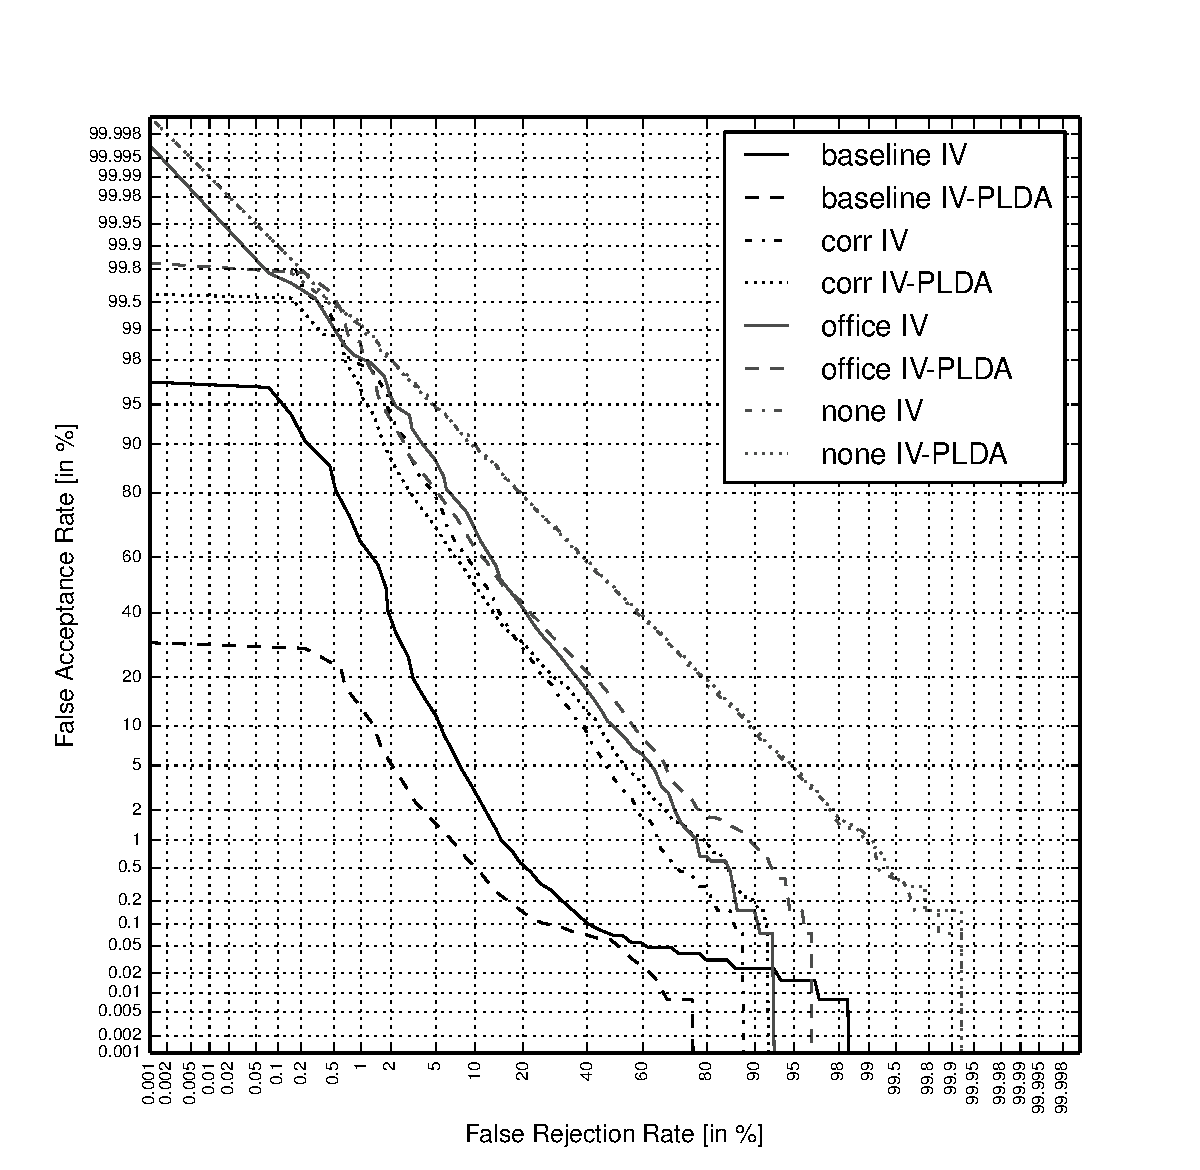
\includegraphics[width=1\linewidth]{Figs/DET_PLDA_iPad_Snorm.pdf}
%	\caption{DET plots for replay attack for the ASV based on iVectors with and without PLDA, with score normalisation (a tablet used as a replay device).}
%	\label{fig::DETs_PLDA}
%
%\end{figure}

\subsection{Results of experiments with the replay countermeasure}


\begin{table*}
%\ninept
\begin{center}
    \begin{tabular}{ l || c c c c c }
    \hline
     	 Environment & \% attacks detected & EER no CM & EER with CM & FAR no CM & FAR with CM\\ 

 \hline \hline
Office   & 80.46 & 30.30 & 14.46 & 88.70 & 52.88\\
Corridor & 73.09 & 24.53 & 13.82 & 80.91 & 48.02\\
None & 62.90 & 49.46 & 30.03 & 97.00 & 86.30\\
\hline
    \end{tabular}
    \caption{Replay attack recognition rate, EER and FAR values for various environment of replay attacks, with and without the countermeasure applied. The FAR was measured for FRR equal to the baseline EER (2.98\%), replay recognition rate given for false positive rate of 11.53\%.}
		\label{tab::results_CM_rooms}
   \end{center}
\end{table*}


\begin{table*}
%\ninept
\begin{center}
    \begin{tabular}{ l || c c c c c }
    \hline
     	 Environment & \% attacks detected & EER no CM & EER with CM & FAR no CM & FAR with CM\\ 

 \hline \hline
Smartphone   & 96.01 & 33.96 & 11.47 & 88.38 & 49.31\\
Tablet & 87.82 & 34.48 & 14.58 & 88.42 & 54.93\\
Stand-alone speaker & 32.61 & 35.84 & 32.25 & 89.80 & 82.96\\
\hline
    \end{tabular}
    \caption{Replay attack recognition rate, EER and FAR values for various replay devices used for attacks, with and without the countermeasure applied. The FAR was measured for FRR equal to the baseline EER (2.98\%), replay recognition rate given for false positive rate of 11.53\%.}
		\label{tab::results_CM_spk}
   \end{center}
\end{table*}


The detailed results of experiments with far-field detection countermeasure for various replay environment, averaged across the replay devices, are presented in Table~\ref{tab::results_CM_rooms}. It shows that the countermeasure performance varies depending on acoustic environment. The relative improvement caused by the countermeasure turned out to be the highest for the most difficult case, i.e., when the acoustic conditions are not taken into account -- in this case the EER decreased from almost 50\% down to 30\%. The relative improvement was the lowest for the case where spoofing was initially least successful, i.e. for the corridor -- it decreased from 24\% to less than 14\%. Anyway, after applying the countermeasure, it was for the corridor where the absolute EER value was the lowest, what we believe is caused by the high reverberation of the corridor.

Table~\ref{tab::results_CM_spk}, in contrast, displays the results of the countermeasure experiments for various replay devices, averaged across different acoustic environments. Even though surprisingly the reply devices had no major impact on spoofing effectiveness (all three devices made the IV-PLDA system yield the EER of ca. 35\%), they do have strong impact of effectiveness of reply countermeasure. The far-field detection countermeasure seems to help best for a smartphone and slightly worse for a tablet (the EER values decreased to less than 12\% and 15\%, respectively). However, the countermeasure worked poorly for a stand-alone speaker -- the EER decreased here on average only by ca. 3\%. 

These results may seem somewhat surprising, considering the fact it was the IR of a stand-alone speaker which was used to train the far-field recording detector, while neither any smartphone IR nor any tablet IR were used to create the training corpus. Anyway we believe that the poor detection of replay attacks caused by the stand-alone speaker is caused by high quality of audio playback provided by such speakers (see e.g. much better frequency response for a stand0alone speaker shown in Fig.~\ref{fig::IRs}), what obviously makes reply detection much more difficult (less than one third of attacks detected if no acoustic conditions considered, at the level of 11.5\% of false rejections). 

Even though the countermeasure applied detected more than 90\% of replay attacks when using a smartphone and a tablet (at the level of 11.5\% of false rejections), and the EER and also FAR values decreased significantly, the FAR values at the false rejection rate set to baseline EER (2.98\%) remain still high (e.g., 49\% for a smartphone and 54\% for a tablet). This is also confirmed by the shape of DET plots presented in Fig~\ref{fig::DETs_CM}. This, however, can be modified within certain limits by adjusting the threshold of the far-field recording classifier.

%% DETs w/wo CM
\begin{figure}
	\centering
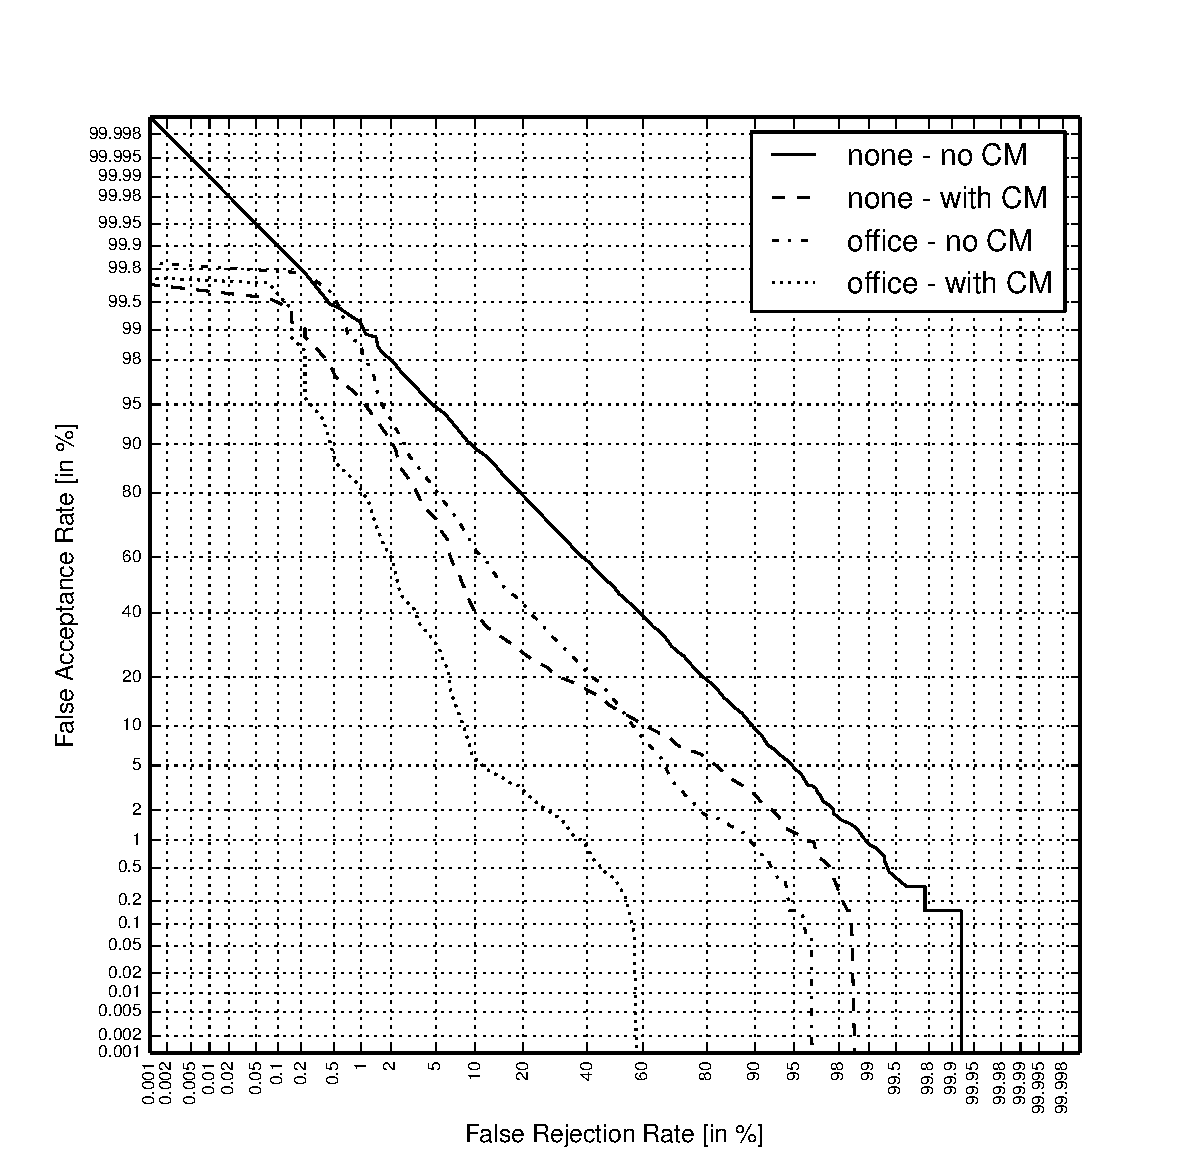
\includegraphics[width=1\linewidth]{Figs/DET_IVPLDA_counter_vil3_iPad.pdf}
	\caption{DET plots for IV-PLDA system for various replay environments, with and without the countermeasure.}
	\label{fig::DETs_CM}
\end{figure}


%% EER w/wo CM
%\begin{figure}
%	\centering
%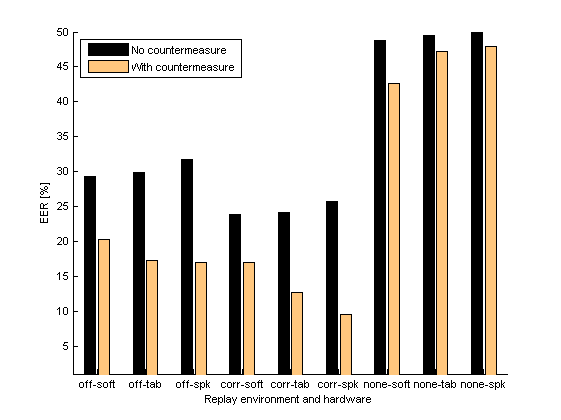
\includegraphics[width=1\linewidth]{Figs/EER_CM.png}
%	\caption{EER results for IV-PLDA under replay attack  with and without countermeasure applied.}
%	\label{fig:EER_PLDA}
%\end{figure}
